\documentclass[main.tex]{subfiles}

\begin{document}

\chapter{Sistemi planetari.}
\PartialToc

\section{Classificazione.}

\subsection{Definizione pianeta (IAU).}

Un pianeta ha le seguenti caratteristiche
\begin{itemize}
    \item \'E in orbita attorno ad una stella di riferimento.
    \item \'E abbastanza massiccio da essere dominato dalle forze di gravit\'a: forma di equilibrio ''idrostatica''.
    \item Ha completamente ripulito la regione del sistema intorno alla sua orbita. Altrimenti \'e un pianeta nano.
\end{itemize}

\section{Luminosit\'a di un pianeta.}

Un pianeta \'e caratterizzato da emissione nel visibile e nell'infrarosso: dell'energia radiante ricevuta da un'eventuale stella parte viene riflessa e parte assorbita e riemessa nell'infrarosso.

\begin{figure}[!ht]
\centering
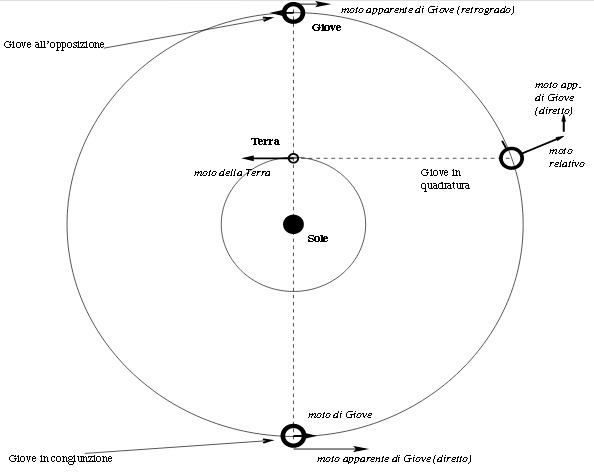
\includegraphics[width=(0.8\textwidth),height=\textheight,keepaspectratio]{apparentJ}
\caption{Configurazioni pianeta/stella.}
\end{figure}


\subsection{Albedo.}

Un pianeta di raggio $R_P$ a distanza dalla stella $r_{P*}^2$ riceve
\begin{align*}
    &\Lambda_{\lambda,P}=\frac{L_{\lambda}^*\pi R_P^2}{4\pi r_{P*}^2}\\
    &0.25L_{\lambda}^*\frac{R_P^2}{r_{P*}^2}
\end{align*}

se riflette una percentuale $A_{\lambda}$ (albedo) la sua luminosit\'a monocromatica (emisfero illuminato) \'e
\begin{align*}
&L_{\lambda,P}=A_{\lambda}\Lambda_{\lambda,P}\\
&L_P=\int_{Vis.}A_{\lambda}\Lambda_{\lambda,P}=A\int_{Vis}\Lambda_{\lambda,P}\,d\lambda
\end{align*}

quindi per un pianeta all'opposizione si ha
\begin{align*}
&I_V=\int_{Vis}\frac{S_V(\lambda)D_{\lambda}(\theta) L_{\lambda,P}}{4\pi r_{P,T}^2}\,d\lambda\\
&=\int_{Vis}\frac{S_V(\lambda)D_{\lambda}(\theta) A_{\lambda}L_{\lambda}^*R_P^2}{14\pi^2r_{P,T}^2r_{P*}^2}\,d\lambda\\
&r_{PT}=r_{P*}-r_{T*}
\end{align*}

\subsection{Magnitudine di un pianeta.}

\begin{align*}
&m_V=-2.5\log{I_V}+\const{}\\
&=-2.5\log{(\int S_V(\lambda)D_{\lambda}(\theta)A_{\lambda}L_{\lambda}^*\,d\lambda)}\\
&-5\log{R_P}+5\log{r_{PT}}+5\log{r_{P*}}+\const{}\\
&=-2.5\log{(\int S_V(\lambda)D_{\lambda}(\theta)A_{\lambda}L_{\lambda}^*\,d\lambda)}\\
&-5\log{(\sqrt{A'}R_P)}+5\log{r_{PT}}+5\log{r_{P*}}\\
&+\const{}
\end{align*}

Per un pianeta molto lontano dalla stella ($r_{T*}\ll r_{P*}$)
\begin{align*}
&m_V=m_{V_0}+10\log{r_{PT}}&\intertext{$m_{V_0}$ indipendente dalla distanza.}
\end{align*}

\subsection{Energia assorbita. Temperatura efficace.}

Suppongo una distribuzione uniforme sulla superficie del pianeta.

La temperatura efficace del pianeta nell'approssimazione di corpo nero
\begin{align*}
&4\pi R_P^2\sigma T_{eff,P}^4=(1-A)\frac{L^*R_P^2}{4r_{P*}^2}\\
&=(1-A)\frac{\pi R_*^2T_{eff,*}^4}{r_{P*}^2}R_P^2\\
&T_{eff,P}=(\frac{1-A}{A})\expy{\frac{1}{4}}(\frac{R_*}{r_{P*}})\expy{\frac{1}{2}}T_{eff,*}
\end{align*}

Approssimazioni successive
\begin{itemize}
    \item Correzione all'approssimazione di corpo nero: corpo grigio. Tengo conto degli effetti di riflessione (corpo nero: assorbimento perfetto).
    \item Differenza di temperatura tra regioni illuminate e non del pianeta: modello termico. Regioni polari meno illuminate cio\'e pi\'u fredde: \'e vero se l'asse di rotazione \'e ortogonale al piano dell'orbita (non vale per Urano).
    
    Per corpi con rotazione veloce o con atmosfera l'escursione termica \'e modesta.
    
    Equilibrio termico locale. Nel punto della superficie in cui il Sole \'e allo zenit: $T_{s*}=(\frac{R_*}{r_{P*}})\expy{\frac{1}{2}}T_{eff,*}$.
\end{itemize}


\section{Il sistema solare.}
Il Sistema Solare: scoperta e osservazione di corpi planetari. magnitudine di un pianeta; osservazioni nel visibile; albedo. Luce riemessa nell'infrarosso; stime di temperatura e modelli termici.
I pianeti: definizione e caratteristiche generali.
I pianeti nani e i corpi minori 
I corpi minori (conclusione). 

Spostandosi verso i pianeti pi\'u esterni il moto proprio decresce sia per la maggiore distanza sia per la minore velocit\'a orbitale. La parallasse diminuisce solo per la maggiore distanza.

\subsection{Giove.}

Il diametro di Giove $D_G\approx\SI{e5}{\kilo\meter}$ visto dalla terra sottende angolo \mblock{\alpha\approx\SI{1.5e-4}{\radian}=\ang{;;30}}. 

\begin{figure}[!ht]
\centering
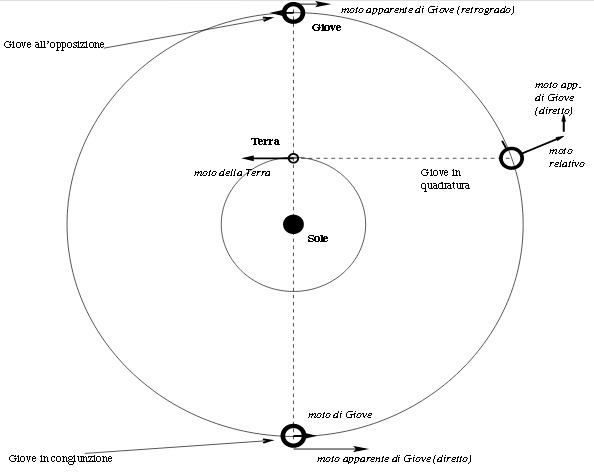
\includegraphics[width=(\textwidth),height=(0.9\textheight),keepaspectratio]{apparentJ}
\caption{Moto reale e apparente nel sistema J/E/S.}
\end{figure}

Caratteristiche dell'orbita:
\begin{itemize}
    \item $\Pi_{360}\approx\SI{12}{\year}$.
    \item $d_{G\odot}\approx\SI{5}{\astronomicalunit}$.
    \item $e=0.048$ ($d(P,F)=ed(P,r), b^2=(1-e^2)a^2$)
\end{itemize}

\subsection{Pianeti Maggiori.}

\begin{figure}[!ht]
\centering
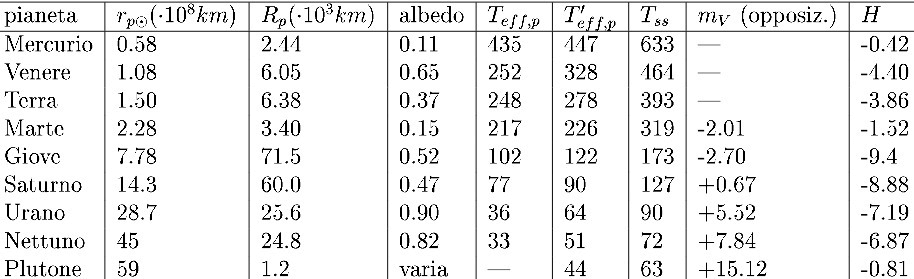
\includegraphics[width=(\textwidth),height=(0.9\textheight),keepaspectratio]{pianetiSS}
\caption{Pianeti maggiori sistema solare.}
\end{figure}

\begin{figure}[!ht]
\centering
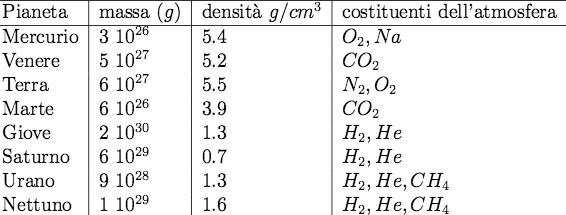
\includegraphics[width=(0.8\textwidth),height=\textheight,keepaspectratio]{systempmass}
\caption{Masse e composizione pianeti maggiori.}
\end{figure}

\subsection{Corpi minori.}

\begin{itemize}
    \item Satelliti
    \item Anelli
    \item Asteroidi, comete, TNO, ogetti della fascia di Kuiper-Edgeworth.
\end{itemize}

Forniscono informazioni sui processi di formazione del sistema solare.

\subsubsection{Evoluzione del sistema solare.}

Approccio statistico: processi collisionali e dinamici.

\subsubsection{Asteroidi.}

Orbite comprese tra Marte e Giove. Il primo \'e 1Ceres, diametro circa \SI{1000}{\kilo\meter}.

Da Terra si vedono come sorgenti puntiformi. Forma, dimensioni e caratteristiche superficiali: tecniche interferometriche e fenomeni di occultamento.

La spettro di riflessione \'e vario: dipende dalle caratteristiche chimiche e fisiche della superficie.

Sono la principale sorgente di meteoriti.

Classificazione in base a indici di colore (fotometria multibanda):
\begin{itemize}
    \item C: Condriti carbonacee.
    \item S: asteroidi con bassa albedo
\end{itemize}

Classificazione dinamica:
\begin{itemize}
    \item Fascia principale: tra Marte e Giove.
    \item Rapido spopolamento man mano che ci si avvicina a Giove.
    \item Lacune di Kirkwood: per valori del semi-asse maggiore risonanti con quello di Giove
    (Risonanza: rapporto periodo orbitale razionale non troppo distante da 1.).
    
    \begin{definition}{Risonanze orbitali}
    In celestial mechanics, an orbital resonance occurs when two orbiting bodies exert a regular, periodic gravitational influence on each other, usually due to their orbital periods being related by a ratio of two small integers. The physics principle behind orbital resonance is similar in concept to pushing a child on a swing, where the orbit and the swing both have a natural frequency, and the other body doing the "pushing" will act in periodic repetition to have a cumulative effect on the motion. Orbital resonances greatly enhance the mutual gravitational influence of the bodies, i.e., their ability to alter or constrain each other's orbits. In most cases, this results in an unstable interaction, in which the bodies exchange momentum and shift orbits until the resonance no longer exists. Under some circumstances, a resonant system can be stable and self-correcting, so that the bodies remain in resonance. Examples are the $1:2:4$ resonance of Jupiter's moons Ganymede, Europa and Io, and the $2:3$ resonance between Pluto and Neptune. Unstable resonances with Saturn's inner moons give rise to gaps in the rings of Saturn. The special case of 1:1 resonance (between bodies with similar orbital radii) causes large Solar System bodies to eject most other bodies sharing their orbits; this is part of the much more extensive process of clearing the neighbourhood, an effect that is used in the current definition of a planet.

A binary resonance ratio in this article should be interpreted as the ratio of number of orbits completed in the same time interval, rather than as the ratio of orbital periods, which would be the inverse ratio. Thus the 2:3 ratio above means Pluto completes two orbits in the time it takes Neptune to complete three. In the case of resonance relationships between three or more bodies, either type of ratio may be used (in such cases the smallest whole-integer ratio sequences are not necessarily reversals of each other) and the type of ratio will be specified.
    \end{definition}
\end{itemize}

\subsection{Tipi di risonanze orbitali}

In general, an orbital resonance may

    involve one or any combination of the orbit parameters (e.g. eccentricity versus semimajor axis, or eccentricity versus orbital inclination).
    act on any time scale from short term, commensurable with the orbit periods, to secular, measured in 104 to 106 years.
    lead to either long-term stabilization of the orbits or be the cause of their destabilization.

A mean-motion orbital resonance occurs when two bodies have periods of revolution that are a simple integer ratio of each other. Depending on the details, this can either stabilize or destabilize the orbit. Stabilization may occur when the two bodies move in such a synchronised fashion that they never closely approach. For instance:

    The orbits of Pluto and the plutinos are stable, despite crossing that of the much larger Neptune, because they are in a 2:3 resonance with it. The resonance ensures that, when they approach perihelion and Neptune's orbit, Neptune is consistently distant (averaging a quarter of its orbit away). Other (much more numerous) Neptune-crossing bodies that were not in resonance were ejected from that region by strong perturbations due to Neptune. There are also smaller but significant groups of resonant trans-Neptunian objects occupying the 1:1 (Neptune trojans), 3:5, 4:7, 1:2 (twotinos) and 2:5 resonances, among others, with respect to Neptune.
    In the asteroid belt beyond 3.5 AU from the Sun, the 3:2, 4:3 and 1:1 resonances with Jupiter are populated by clumps of asteroids (the Hilda family, the few Thule asteroids, and the extremely numerous Trojan asteroids, respectively).

Orbital resonances can also destabilize one of the orbits. For small bodies, destabilization is actually far more likely. For instance:

    In the asteroid belt within 3.5 AU from the Sun, the major mean-motion resonances with Jupiter are locations of gaps in the asteroid distribution, the Kirkwood gaps (most notably at the $3:1$, $5:2$, $7:3$ and $2:1$ resonances). Asteroids have been ejected from these almost empty lanes by repeated perturbations. However, there are still populations of asteroids temporarily present in or near these resonances. For example, asteroids of the Alinda family are in or close to the $3:1$ resonance, with their orbital eccentricity steadily increased by interactions with Jupiter until they eventually have a close encounter with an inner planet that ejects them from the resonance.
    In the rings of Saturn, the Cassini Division is a gap between the inner B Ring and the outer A Ring that has been cleared by a $2:1$ resonance with the moon Mimas. (More specifically, the site of the resonance is the Huygens Gap, which bounds the outer edge of the B Ring.)
    In the rings of Saturn, the Encke and Keeler gaps within the A Ring are cleared by 1:1 resonances with the embedded moonlets Pan and Daphnis, respectively. The A Ring's outer edge is maintained by a destabilizing $7:6$ resonance with the moon Janus.

Most bodies that are in resonance orbit in the same direction; however, a few retrograde damocloids have been found that are temporarily captured in mean-motion resonance with Jupiter or Saturn. Such orbital interactions are weaker than the corresponding interactions between bodies orbiting in the same direction.

A Laplace resonance is a three-body resonance with a 1:2:4 orbital period ratio (equivalent to a $4:2:1$ ratio of orbits). The term arose because Pierre-Simon Laplace discovered that such a resonance governed the motions of Jupiter's moons Io, Europa, and Ganymede. It is now also often applied to other 3-body resonances with the same ratios, such as that between the extrasolar planets Gliese 876 c, b, and e. Three-body resonances involving other simple integer ratios have been termed "Laplace-like" or "Laplace-type".

A Lindblad resonance drives spiral density waves both in galaxies (where stars are subject to forcing by the spiral arms themselves) and in Saturn's rings (where ring particles are subject to forcing by Saturn's moons).

A secular resonance occurs when the precession of two orbits is synchronised (usually a precession of the perihelion or ascending node). A small body in secular resonance with a much larger one (e.g. a planet) will precess at the same rate as the large body. Over long times (a million years, or so) a secular resonance will change the eccentricity and inclination of the small body.

Several prominent examples of secular resonance involve Saturn. A resonance between the precession of Saturn's rotational axis and that of Neptune's orbital axis (both of which have periods of about 1.87 million years) has been identified as the likely source of Saturn's large axial tilt ($26.7\deg$). Initially, Saturn probably had a tilt closer to that of Jupiter ($3.1\deg$). The gradual depletion of the Kuiper belt would have decreased the precession rate of Neptune's orbit; eventually, the frequencies matched, and Saturn's axial precession was captured into the spin-orbit resonance, leading to an increase in Saturn's obliquity. (The angular momentum of Neptune's orbit is 104 times that of Saturn's spin, and thus dominates the interaction.)

The perihelion secular resonance between asteroids and Saturn  helps shape the asteroid belt. Asteroids which approach it have their eccentricity slowly increased until they become Mars-crossers, at which point they are usually ejected from the asteroid belt by a close pass to Mars. This resonance forms the inner and "side" boundaries of the asteroid belt around 2 AU, and at inclinations of about $20\deg$.

Numerical simulations have suggested that the eventual formation of a perihelion secular resonance between Mercury and Jupiter has the potential to greatly increase Mercury's eccentricity and possibly destabilize the inner Solar System several billion years from now.

The Titan Ringlet within Saturn's C Ring represents another type of resonance in which the rate of apsidal precession of one orbit exactly matches the speed of revolution of another. The outer end of this eccentric ringlet always points towards Saturn's major moon Titan.

A Kozai resonance occurs when the inclination and eccentricity of a perturbed orbit oscillate synchronously (increasing eccentricity while decreasing inclination and vice versa). This resonance applies only to bodies on highly inclined orbits; as a consequence, such orbits tend to be unstable, since the growing eccentricity would result in small pericenters, typically leading to a collision or (for large moons) destruction by tidal forces.

In an example of another type of resonance involving orbital eccentricity, the eccentricities of Ganymede and Callisto vary with a common period of 181 years, although with opposite phases.

\subsubsection{Troiani.}

Sono oggetti che hanno lo stesso semi-asse di Giove ma spostati di \ang{+-60} nell'orbita cio\'e nei punti Lagrangiani.

\subsubsection{NEA/NEO.}

Orbita pi\'u interna, incrocia anche l'orbita della Terra.

\subsubsection{Comete.}
Orbite eccentriche.

Il cambiamento delle loro propriet\'a dipende dalla distanza dal Sole: ricche di sostanze volatili

Originaria di una fascia esterna di corpi minori compresa tra asteroidi e TNO, in seguito a incontri ravvicinati con corpi maggiori si sono spostate in orbite che raggiungono all'afelio i confini del sistema solare (Nube di Oort approx \SI{e5}{\astronomicalunit}: quando diventa prevalente l'attrazione delle stelle vicine).

\subsubsection{Centauri.}

Centauri: orbite comprese tra Giove e Nettuno. La zona \'e dinamicamente instabile e porta in orbite cometaria.

\subsubsection{Trans-Neptunian object: Fascia di Kuiper-Edgeworth.}

Oltre Nettuno di hanno i TNO.

Un sottogruppo dei TNO, i plutini, sono in risonanza $3:2$ con Nettuno (come Plutone).

\subsection{Search motivation}

\begin{itemize*}
\item Why acretional formation of solar system planet objects should stop at Neptuno's distance.
\item The jupiter family comets are almost on planar orbits with low inclination on ecliptic plane (plane of solar system). This is inesplicable if the source is far away and isotropic, so we may may postulate a a disc of cometary object beyond Neptun.
\end{itemize*}

\clearpage

\section{Interplanetary materials and meteorites}

\subsection{Comets}

\subsection{Asteroids}

\subsection{Short summary}
\begin{itemize*}
\item Originate from primitive bodies: TNO, comets and asteroids.
\item Span 20 order of magnitude in mass
\item Observed ground or space based optically or IR: reflected solar light or thermal emission by small interplanetary dust arranged in a disk like structure on the ecliptic plane.
Zodiacal light is caused by reflected light at large angle, false corona light is attributed to small angle diffractive scattering.
\end{itemize*}



\section{Grandezze caratteristiche del sole.}

\subsection{Et\'a del sole. Evolouzione pre-sequenza principale.}

\subsubsection{Datazione Meteoriti}

Per datare i meteoriti si usa il decadimento $^{87}Rb\to^{87}Sr$ con $\thalf=4.8\sci{10}\,yr$ o altri processi. La maggior parte dei meteoriti si sono formati nel disco di accrescimento ed hanno un'et\'a di $T=(4.55\pm0.05)\sci{9}\,yr$.


\subsubsection{Modello formazione sistema solare. Nascita proto-stella.}

\'E possibile mettere in relazione l'et\'a dei meteoriti con l'inizio della fase di sequenza principale del sole grazie ai modelli di formazione del sistema solare.
Il collasso di una nube di miglia di masse solari molto rarefatta \'e govarnato dal criterio di Jeans

\begin{equation}\label{eq:cjeans}
\frac{Gm(r)}{r}>\frac{RT}{\mu}
\end{equation}

In questo caso la nube si contrae con un tempo caratteristico $\tff=(\overline{\rho}G)\expy{-\frac{1}{2}}\approx\sci{7}\,yr$ e  il criterio di Jeans \'e verificato in sub-zone quindi la nube iniziale si  frammenta spontaneamente.

La materia del sottosistema che porter\'a alla formazione di una stella tipo Sole in seguito al collasso gravitazionale 

si addensa un core centrale in equilibrio idrostatico e il resto della materia forma un disco di accrescimento in free fall verso il core denso. Nel disco di accrescimento, per il tempo impiegato dalla disco a confluire sulla stella, ordine di $\sci{6}\,yr$, si sono formati la maggior parte dei meteoriti.~\ref{eq:cjeans}

\subsubsection{Inizio processi di fusione. Tempo in sequenza principale}

La luminosit\'a della protostella \'e alimentata dal collasso gravitazionale: dal teorema del viriale risulta che met\'a dell'energia gravitazionale guadagnata per unit\'a di tempo alimenta la luminosit\'a della proto-stella l'altra met\'a ne aumenta l'energia termica. Il tempo necessario perch\'e si raggiungano nella zona centrale densit\'a e temperature sufficienti per le reazioni di fusione \'e dell'ordine  del tempo-scala di \kh{}, $\tkh{}=\frac{Gm^2}{rL}$. 


\begin{figure}[!ht]
\centering
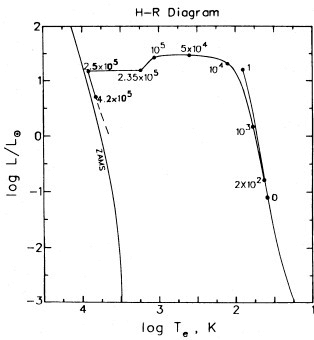
\includegraphics[width=(0.8\textwidth),height=\textheight,keepaspectratio]{premain}
\caption{Evoluzione verso inizio reazioni fusione.}
\end{figure}


Il risultato della differenza tra l'et\'a del sistema solare e il tempo impiegato dal collasso a raggiungere le condizioni per la fusione dell'idrogeno \'e il periodo trascorso dal sole in sequenza principale:

L'et\'a del sole \'e $\tsun=(4.566\pm0.005)*\sci{9}\,yr$.



\subsection{Distanza, Massa, Raggio e Luminosit\'a.}

\subsubsection{Distanza}


Il prodotto $G\msun$ \'e determinato da moti planetari quindi $\msun1.989*\sci{33}\,gr$.
\index{Distanza (fare) moderni?}

\subsubsection{Raggio}

La determinazione del raggio solare si riduce alla misura del  diametro apparente e ad un modello della regione di transizione: nota la distanza terra-sole ho una misura di $\rsun$,  un valore  rappresentativo \'e $\rsun=6.9599\sci{10}\,cm=695.99\,Mm$. Per correzioni vedi parte di inversione.

\subsubsection{Luminosit\'a}
La luminosit\'a solare misurata tramite satelliti risultante dalla media in un ciclo solare $\lsun=3.846*\sci{33}\,erg\,s^{-1}$.


\subsection{Composizione}

Caratterizzo la composizione stellare attraverso X, Y, Z che rappresentano rispettivamente abbondanza in massa di idrogeno ,elio ed elementi pesanti. Le misure spettroscopiche danno risultati accurati per elementi pi\'u pesanti dell'elio. Le linee di assorbimento dell'elio sono presenti solo negli strati superiori dell'atmosfera solare a causa delle alte energie di eccitazione. Misuro invece il rapporto $\frac{Z_s}{X_s}$ che caratterizza la composizione attuale della superficie: ho che $\frac{Z_s}{X_s}=0.0245-0.23$.




\chapter{Sistemi planetari extrasolari.}
Sistemi planetari extrasolari: introduzione.
 Sistemi extrasolari: tecniche di scoperta. 
Le caratteristiche generali dei sistemi extrasolari conosciuti. Problemi aperti. Il problema dell'abitabilita' e della ricerca della vita nell'Universo (cenni). Introduzione all'astrofisica extragalattica.L'universo: la legge di Hubble e il Big Bang (introduzione). 
Il "modello standard" di universo, e sua crisi. Teorie inflazionarie (cenni).
Distribuzione di massa su grande scala. Funzioni di correlazione. tecniche di analisi statistica: la percolazione.
\PartialToc

Distinzione pianeta/brown dwarf: $M_P\leq20M_J$, i pianeti veri e propri hanno masse $M_P\leq13M_J$.

Domande fondamentali:
\begin{itemize}
    \item Quanto \'e frequente la formazione di sistemi planetari all'atto di formazione stellare?
    \item Quanto \'e frequente la formazione di pianeti terrestri?
    \item Quanto \'e frequente la nascita della vita?
\end{itemize}

\begin{figure}[!ht]
\centering
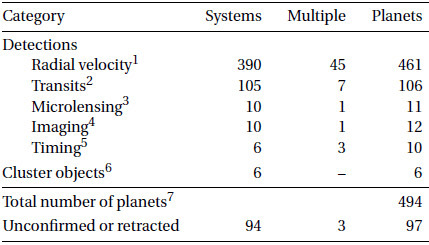
\includegraphics[width=(0.7\textwidth),height=\textheight,keepaspectratio]{exostats}
\caption{Exoplanet detection statistic (2010).}
\end{figure}

\clearpage

\section{Moto dei pianeti.}


\begin{figure}[!ht]
\centering
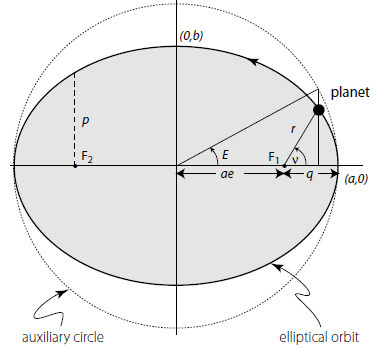
\includegraphics[width=(0.7\textwidth),height=\textheight,keepaspectratio]{orbits}
\caption{orbits.}
\end{figure}

\subsection{Moto attorno al centro di massa}

Il moto di un singolo pianeta attorno ad una stella provoca un moto riflesso della stella attorno al centro di massa. Questo provoca perturbazione delle caratteristiche osservabili
\begin{itemize}
    \item Radial velocity
    \item angular (astrometric) position in the sky
    \item arrival time of periodic reference signal 
\end{itemize}

Il pianeta e la stella orbitano attorno al comune CM in orbite ellittiche chiuse con il CM come uno dei 2 fuochi.

\begin{align*}
&r=\frac{a(1-e^2)}{1+e\cos{\nu}}\\
&\frac{x^2}{a^2}+\frac{y^2}{b^2}=1\\
&b^2=a^2(1-e^2)
\end{align*}

\subsection{Anomali vera, eccentrica e media.}

Anomalia vera, $\nu(t), f(t)$: \'e l'angolo tra la direzione del pericentro e la posizione al tempo t misurata dal baricentro. L'anomalia eccentrica \'e l'angolo corrispondente all'anomalia vera riferito al cerchio ausiliario
\begin{align*}
&\cos{\nu(t)}=\frac{\cos{E(t)}-e}{1-e\cos{E(t)}}\\
&\tan{\frac{\nu(t)}{2}}=\sqrt{\frac{1+e}{1-e}}\tan{\frac{E(t)}{2}}
\end{align*}

L'anomalia medi \'e un'angolo relativo al moto medio attorno all'orbita: in un'orbita completa il pianeta non ha velocit\'a angolare costante ma una velocit\'a angolare media \'e specificata in termini del moto medio $n=\frac{2\pi}{P}$. L'anomalia media al tempo $t-t_p$ dopo il passaggio al pericentro \'e
\begin{align*}
&M(t)=\frac{2\pi}{P}(t-t_p)=n(t-t_p)\\
&M(t)=E(t)-e\sin{E(t)}
\end{align*}

\subsection{Specificazione dell'orbita.}

\begin{figure}[!ht]
\centering
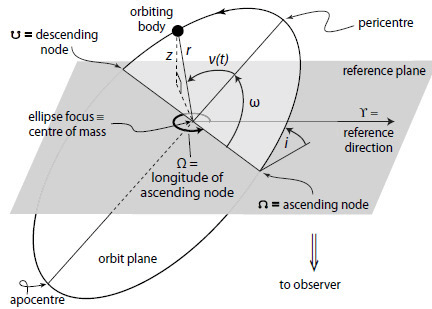
\includegraphics[width=(0.7\textwidth),height=\textheight,keepaspectratio]{orbits3D}
\caption{Keplerian orbit description in 3D.}
\end{figure}

\clearpage

\subsection{Leggi di Keplero}

\begin{figure}[!ht]
\centering
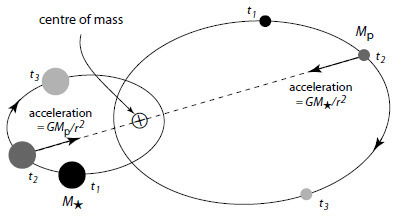
\includegraphics[width=(0.7\textwidth),height=\textheight,keepaspectratio]{orbitsCM}
\caption{Two orbiting bodies.}
\end{figure}

Leggi di keplero (Original)

\begin{enumerate*}
    \item L'orbita di un pianeta \'e un'ellisse con il Sole come fuoco. (Inverse square law of gravity)
    \item Il raggio che congiunge Sole-pianeta spazza aree uguali in intervalli uguali. (Conservazione momento angolare)
    \item Il quadrato del periodo orbitale dei pianeti \'e proporzionale al cubo del semiasse maggiore. (Inverse square law of gravity)
\end{enumerate*}

Quando la massa del pianeta non \'e trascurata
\begin{equation*}
    P^2=\frac{4\pi^2}{GM}a^3
\end{equation*}

Specifico:
\begin{itemize}
    \item Orbite relative: moto del pianeta relativo alla stella.
    \begin{equation*}
    P^2=\frac{4\pi^2}{G(M_*+M_p)}a^3_{Rel}
    \end{equation*}
    dove usiamo il semiasse maggiore dell'orbita relativa.
    
    Per $M_P\ll M_*$ in unit\'a dell'orbita terrestre
    \begin{equation*}
    P\approx\SI{1}{\year}(\frac{a_{Rel}}{\si{\astronomicalunit}})\expy{\frac{3}{2}}(\frac{M_*}{\msun{}})\expy{-\frac{1}{2}}
    \end{equation*}
    
    \item Orbite assolute: per l'orbita della stella attorno al baricentro del sistema vale
    \begin{equation*}
    P^2=\frac{4\pi^2}{GM'}a_*^3
    \end{equation*}
    dove $M'=\frac{M_P^3}{(M_*+M_P)^2}$ e $a_*$ \'e il semi-asse maggiore dell'orbita stellare attorno al baricentro.
    
    Espressione equivalente per l'orbita del pianeta attorno al baricentro.
    
    Le dimensioni delle orbite sono in proporzione:
    \begin{equation*}
        a_*:a_p:a_{rel}=M_p:M_*:(M_p+M_*)
    \end{equation*}
    con $a_{rel}=a_p+a_*$, $P_{rel}=P_p=P_*$ e $e_{rel}=e_p=e_*$.
    
\end{itemize}



\clearpage

\section{Metodi per la scoperta di sistemi planetari extrasolari.}

\subsection{Metodi diretti.}

Risoluzione del sistema in maniera visuale: la separazione angolare Sole/Giove sarebbe \SI{1}{\arcsec} gi\'a a \SI{5}{\parsec}.

Estrema differenza tra $L^*$ e $L_P$: per il sistema Sole/Giove nel visibile
\begin{align*}
    \frac{L_P}{L_*}=P(\lambda,\alpha)(\frac{R_P}{a})^2\approx\num{e-9}&\intertext{$P(\lambda,\alpha)$ dipende da albedo e fase a cui si trova il pianeta.}
\end{align*}

Effetto di selezione: pianeti lontani dalla stella ($a>\SI{10}{\astronomicalunit}$).

\subsection{Timing}

Se luce emessa dalla stella primari ha tempi caratteristici il moto ellittico dovuto alla presenza del pianeta produce variazioni nel cammino ottico della luce proporzionaleallo spostamento della primaria lungo la linea di vista
\begin{equation*}
    \tau_p=\frac{1}{c}\frac{a\sin{i}M_p}{M_*}
\end{equation*}

\subsubsection{Osservazioni di pulsar.}

Emettono segnale periodico regolare $\Pi\approx\si{\second}-\si{\milli\second}$. Il moto attorno al comune centro di massa Pulsar/pianeta causa una variazione del cammino ottico: il segnale arriva in anticipo o in ritardo.

Nel caso de lsistema Sole/Terra il sole percorre un'ellisse di semiasse maggiore circa \mblock{\frac{m_T}{\msun{}}a_T\approx\SI{500}{\kilo\meter}}: la differenza di cammino ottico causerebbe un $\Delta t\approx\SI{1}{\milli\second}$.

Sistemi non nati con la stella: formati in fase finale di evoluzione.

\subsection{Microlensing gravitazionale.}

La presenza di materia (densit\'a di energia) distorce lo spazio-tempo e il la radiazione EM pu\'o essere deviata: la luce proveniente da un'oggetto lontano pu\'o essere deviata dal campo gravitazionale di un oggetto (lente) e quindi per l'oservatore risulta distorta e amplificata. 

\begin{definition}{Microlensing.}
Si parla di microlensing quando le immagini multiple dell'oggetto lontano non sono risolte.
\end{definition}

\subsubsection{Gravitational light bending}

\begin{definition}{Raggio di \sch{.}}
Il raggio di \sch{} \'e
\begin{equation*}
    R_S=\frac{2GM_L}{c^2}
\end{equation*}
\end{definition}

\begin{figure}[!ht]
\centering
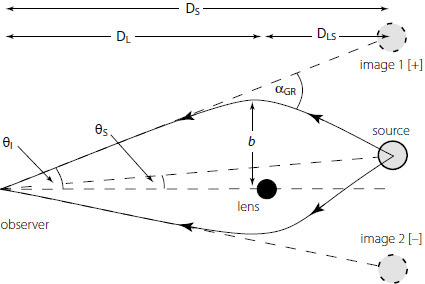
\includegraphics[width=(0.9\textwidth),height=\textheight,keepaspectratio]{lensing}
\caption{lensing.}
\end{figure}

\begin{align*}
&\alpha_{GR}=\frac{4GM_L}{c^2b}=\frac{2R_S}{b}&\intertext{con la condizione che il parametro di impatto $b\gg R_S$}
\end{align*}

Lens equation
\begin{equation*}
\theta_S=\theta_I-2R_S\frac{D_{LS}}{D_LD_S}\frac{1}{\theta_I}
\end{equation*}

\clearpage

\subsubsection{Einstein radius.}

La sorgente lontana vedra la sua luminosit\'a amplificata dalla lente in proporzione all'Anello di Einstein
\begin{equation*}
    \theta_E^2=\frac{4GM_LD_{LS}}{c^2D_{OL}D_{OS}}
\end{equation*}

\begin{figure}[!ht]
\centering
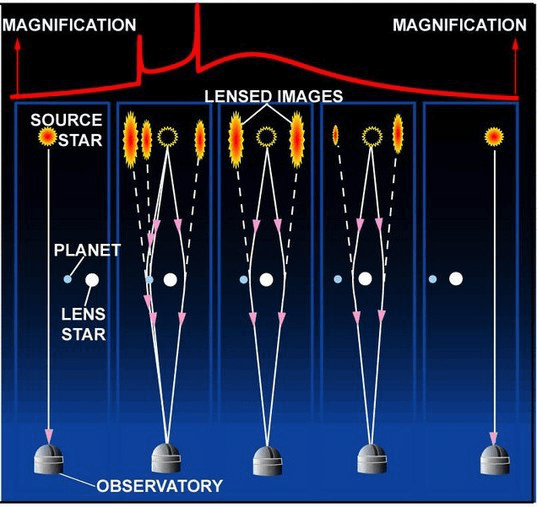
\includegraphics[width=(0.7\textwidth),height=\textheight,keepaspectratio]{microlensing}
\caption{Curva di luce per microlensing.}
\end{figure}

Le sorgenti galattiche possono essere stelle del nucleo galattico ($D_{OS}\approx\SI{10}{\kilo\parsec}$ e lenti tipic a met\'a strada).

Per $M_L\approx\msun{}$: $\theta_E\approx\si{\milli\arcsec}$.

Le dimensioni dell'anello di Einstein definiscono il livello di allineamento richiesto per avere una significativa amplificazione del segnale della sorgente.

Dimensioni lineari dell'anello di Einstein
\begin{align*}
    R_E=(1-y)\,d\theta=\sqrt{2y(1-y)R_Sd}
\end{align*}
con $d=D_{os}$, $yd=D_{LS}$, massime dimensioni lineari per $y=\frac{1}{2}$.
Il raggio di luce deve passare ad una distanza inferiore di $R_E$ dalla lente.

Inserendo quantit\'a tipiche per ricerca di esopianeti
\begin{align*}
&\theta_E\approx1.0(\frac{M_L}{\msun{}})\expy{\frac{1}{2}}(\frac{D_L}{\SI{8}{\kilo\parsec}})\expy{-\frac{1}{2}}(\frac{D_{LS}}{D_S})\expy{\frac{1}{2}}\si{\milli\arcsec}\\
&R_E\approx8.1(\frac{M_L}{\msun{}})\expy{\frac{1}{2}}(\frac{D_S}{\SI{8}{\kilo\parsec}})\expy{\frac{1}{2}}(\frac{D_LD_{LS}}{D_S^2})\expy{\frac{1}{2}}\si{\astronomicalunit}
\end{align*}

\subsubsection{Magnification}

\begin{figure}[!ht]
\centering
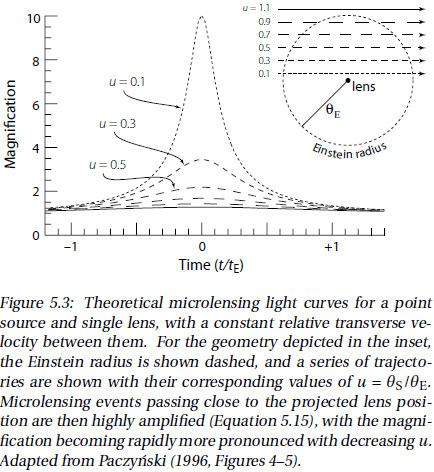
\includegraphics[width=(0.7\textwidth),height=\textheight,keepaspectratio]{lensinglcurves}
\caption{Microlensing magnification.}
\end{figure}

\clearpage

Fatti:
\begin{itemize}
    \item In un cilindro di raggio $R_E$ e altezza $D_{OS}$ ho probabilit\'a $\frac{1}{100000}$ che ci sia una stella.
    \item Se la lente \'e costituita da pi\'u masse avremo una curva di luce con pi\'u picchi
    \item Nel caso di lente con sistema planetario la distribuzione dei picchi \'e detrminata dalla posizione dei pianeti: pi\'u efficace vicino all'anello di Einstein.
\end{itemize}

\begin{figure}[!ht]
\centering
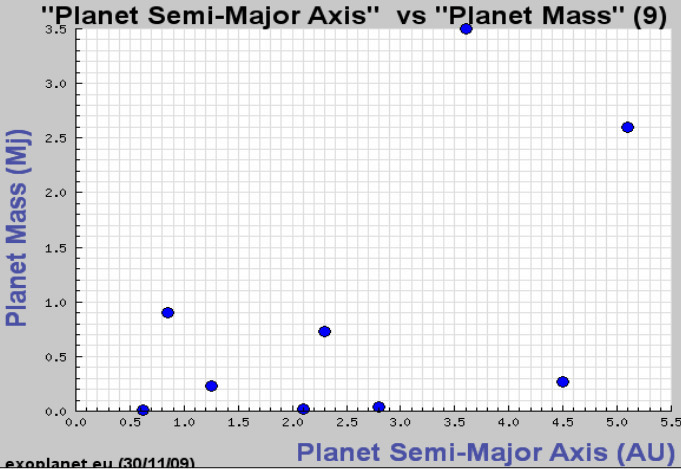
\includegraphics[width=(0.7\textwidth),height=\textheight,keepaspectratio]{mp-a-micro}
\caption{Massa pianeti vs semiasse per pianeti scoperti tramite microlensing.}
\end{figure}

\clearpage

\subsection{Tecniche astrometriche}

Misura posizione e moti dei corpi celesti. The path of a star orbiting star-planet barycentre appears projected on the plane of the sky as an ellipse with angular semi-major axis $\alpha$
\begin{align*}
&a_*:a_{rel}=M_p:(M_p+M_*),\ a_{rel}=a_*+a_p
&\alpha=\frac{M_p}{M_*+M_p}a\approx\frac{M_p}{M_*}a\\
&\approx(\frac{M_p}{M_*})(\frac{a}{\SI{1}{\astronomicalunit}})(\frac{d}{\SI{1}{\parsec}})\expy{-1}\si{\arcsec}
\end{align*}


\subsection{Tecniche spettroscopiche (Misura velocit\'a radiale).}

Variazione periodica della velocit\'a radiale dovuta al moto attorno al CM.

For the radial velocity semi-amplitude we have
\begin{align*}
&v_r=K[\cos{\omega+\nu}+e\cos{\omega}]\\
&K=\frac{2\pi}{T}\frac{A_*\sin{i}}{\sqrt{1-e^2}}\\
&K^2=\frac{G}{(1-e^2)}\frac{1}{a_*\sin{i}}\frac{M_p^3\sin^3{i}}{(M_*+M_p)^2}&\intertext{radial velocity measurement provide a value for mass function}\\
&\frac{M_p^3\sin^3{i}}{(M_*+M_p)^2}
\end{align*}

La terza legge di Keplero
\begin{equation}
(M^*+m_P)\sin^3{i}=\frac{4\pi^2a^3\sin^3{i}}{GP^2}
\end{equation}

$i$ \'e l'inclinazione dell'orbita rispetto al piano nella sfera celeste normale alla linea di vista.

Se entrambi gli spettri fossero osservabili dalle velocit\'a radiali ottengo $a^*\sin{i}, a_P\sin{i}$ e $(M^*+m_P)\sin^3{i}$ essendo $\frac{a^*\sin{i}}{a_P\sin{i}}=\frac{m_P}{m^*}$: ottengo $M^*\sin{i}$ e $m_P\sin{i}$.

Nel caso usuale in cui sia osservabile solo lo spettro della stella:

\begin{align*}
&a=a^*+a_P=a^*(1+\frac{a_P}{a^*})=a^*(1+\frac{M^*}{m_P})\\
&a^3\sin^3{i}=a^*\sin^3{i}(\frac{m_P+M^*}{m_P})^3
\end{align*}

Definisco la funzione delle masse
\begin{align*}
&f(M^*,m_P)=(M^*+m_P)\sin^3{i}\frac{m_P^3}{(M^*+m_P)^3}\\
&=\frac{4\pi^2}{GP^2}{a^*}^3\sin^3{i}\\
&f=\frac{PK_2^3}{2\pi G}&\intertext{$K_2$ is half the change in radial velocity.}\\
&f=\frac{M_1\sin^3{i}}{(1+q)^2}&\intertext{q \'e il rapporto tra le masse $M^*$ fratto massa oggetto non visibile $m_P$.}
\end{align*}

Se il sistema \'e anche fotometrico \'e possibile valutare l'inclinazione; ponendo $i=\frac{\pi}{2}$ ho un limite inferiore per le masse.

Ampiezza variazione velocit\'a radiale massa stella host
\begin{equation*}
v=\frac{30m_P\sin{i}}{{M^*}\expy{\frac{2}{3}}P\expy{\frac{1}{3}}},\ \si{\kilo\meter\per\second}
\end{equation*}
dove la massa \'e espressa in $\msun{}$ e il periodo in anni: posso ricavare $m_P\sin{i}$.

Per il sistema Sole/Giove $v\approx\SI{12}{\meter\per\second}$.

Sole/Terra $v\approx\SI{10}{\cm\per\second}$.

Prendendo la coordinata z della stella lungo la linea di vista
\begin{align*}
&z=r(t)\sin{i}\sin{(\omega+\nu)}\\
&v_r=\dot{z}=K[\cos{(\omega+\nu)}+e\cos{\omega}]\\
&K=\frac{2\pi}{P}\frac{a_*\sin{i}}{(1-e^2)\expy{\frac{1}{2}}}
\end{align*}

\begin{figure}[!ht]
\centering
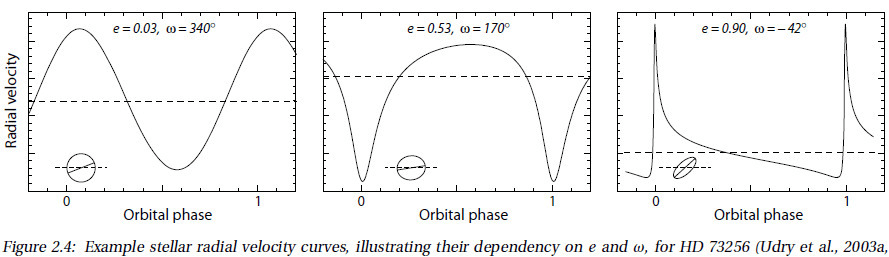
\includegraphics[width=(0.9\textwidth),height=\textheight,keepaspectratio]{vrcurve}
\caption{Stellar radial velocity curves: dependency on $e$ and $\omega$.}
\end{figure}

\clearpage

\subsection{Tecniche fotometriche: transiti.}

\begin{figure}[!ht]
\centering
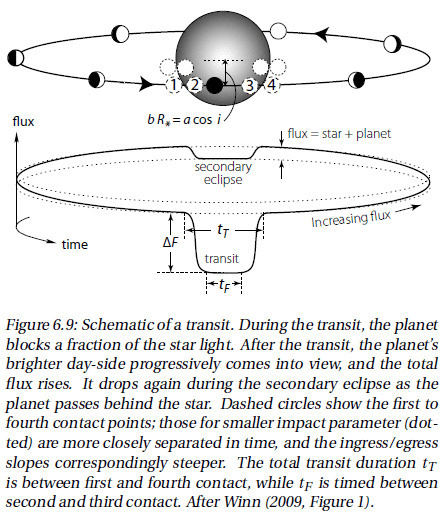
\includegraphics[width=(0.9\textwidth),height=\textheight,keepaspectratio]{transit}
\caption{Schematic of a transit and secondary eclipse (planet passes behind).}
\end{figure}

Abbiamo 4 osservabili
\begin{itemize}
    \item Il periodo P.
    \item La profondit\'a del transito $\Delta F$.
    \item Intervallo di tempo tra 1-4 $t_T$.
    \item Intervallo di tempo tra 2-3 $t_F$.
\end{itemize}


\begin{align*}
&\Delta F\approx(\frac{R_p}{R_*})^2\\
&t_T\approx13(\frac{M_*}{\msun{}})\expy{-\frac{1}{2}}(\frac{a}{\si{\astronomicalunit}})\expy{\frac{1}{2}}\frac{R_*}{\rsun{}}\si{\hour}
\end{align*}

La probabilit\'a che per un pianeta orientato arbitrariamente si possa osservare transito a eclisse secondaria \'e
\begin{equation*}
Pr\frac{R_*}{a}\approx0.005\frac{R_*}{\rsun{}}(\frac{a}{\si{\astronomicalunit}})\expy{-1}
\end{equation*}
data dall'area spazzata dall'ombra del pianeta sulla sfera celeste.

\begin{figure}[!ht]
\centering
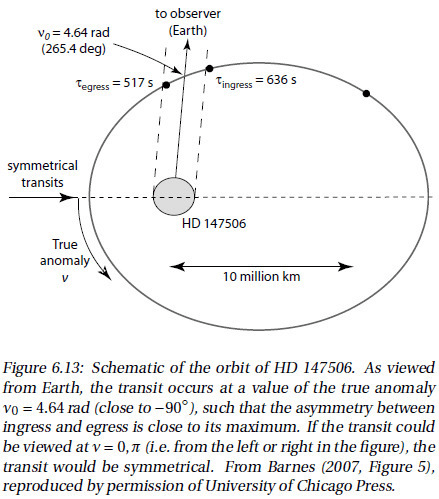
\includegraphics[width=(0.7\textwidth),height=\textheight,keepaspectratio]{transitex}
\caption{Transito visto dalla Terra.}
\end{figure}

\begin{figure}[!ht]
\centering
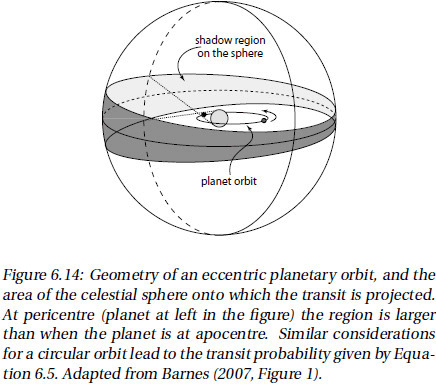
\includegraphics[width=(0.7\textwidth),height=\textheight,keepaspectratio]{sphereshadow}
\caption{Area della sfera celeste su cui \'e proiettato il transito.}
\end{figure}

Fatti:
\begin{itemize}
    \item Per un'eclissi totale Sole/Giove ho variazione $\Delta L\approx1\%$.
\end{itemize}

\begin{figure}[!ht]
\centering
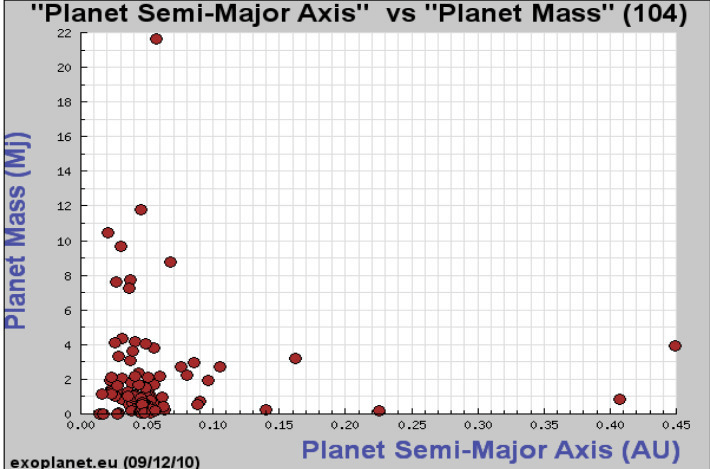
\includegraphics[width=(0.7\textwidth),height=\textheight,keepaspectratio]{mp-atransit}
\caption{Massa pianeta vs semiasse per pianeti scoperti tramite transito.}
\end{figure}

\clearpage

\section{Caratteristiche e problemi interpretativi.}

\begin{figure}[!ht]
\centering
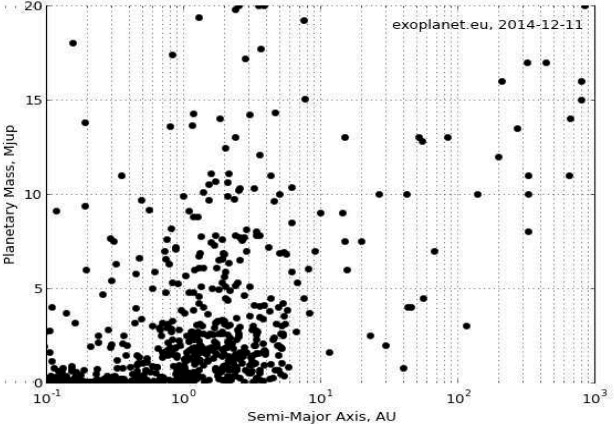
\includegraphics[width=(0.7\textwidth),height=\textheight,keepaspectratio]{mp-a}
\caption{Massa pianeti vs semiasse .}
\end{figure}

\subsection{Caratteristiche preferenziali della stella primaria??}

\begin{equation*}
\frac{\parbox{0.8\textwidth}{$\#$ Sistemi osservati che hanno pianeti}}{\parbox{0.8\textwidth}{$\#$ Sistemi osservati}}
\end{equation*}

''A livello preliminare si oserva una carenza di pianetti attorno a stelle doppie.''

Ci sono caratteristiche delle stelle che rendono pi\'u probabile la formazione di pianeti?

\begin{figure}[!ht]
\centering
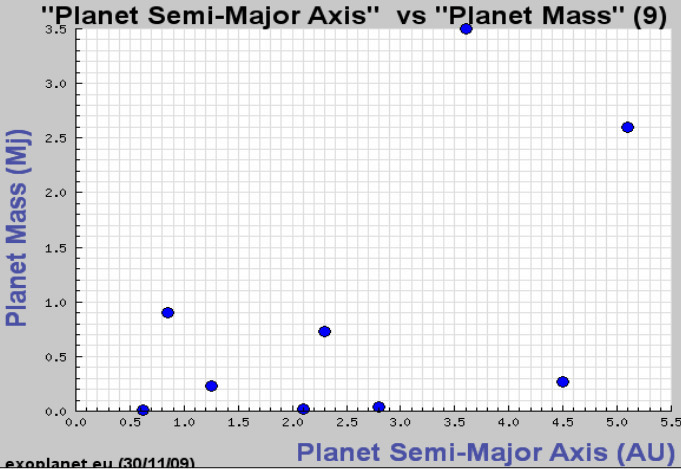
\includegraphics[width=(0.8\textwidth),height=\textheight,keepaspectratio]{mp-a-micro}
\caption{Massa stella primaria.}
\end{figure}

\begin{figure}[!ht]
\centering
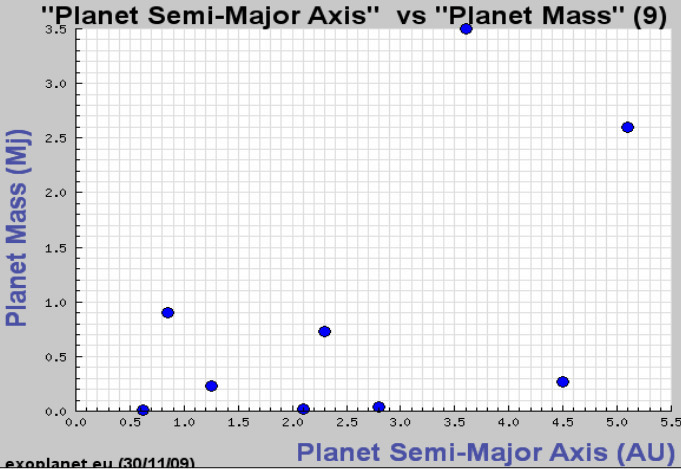
\includegraphics[width=(0.8\textwidth),height=\textheight,keepaspectratio]{mp-a-micro}
\caption{Metallicit\'a stella primaria.}
\end{figure}

\clearpage

\subsection{Modello formazioni pianeti di Sovronof.}

Formazione pianeti a partire da grani solidi della nube proto-planetaria: privilegia sistemi ad alta metallicit\'a, daltra parte l'alta metallicit\'a della stella potrebbe essere causata dalla caduta di materia (pianeti) su di essa.

Pianeti attorno a stelle con bassa metallicit\'a indicherebbe la presenza di pi\'u canali di formazione.

Effetti di selezione: stelle con $M^*<\msun{}$ sono studiate di meno.


\subsection{Distribuzione di massa dei pianeti.}

La distribuzione di massa dei pianeti \'e piccata attorno a $M_J$ e il $60\%$ dei pianeti hanno massa $m_P<2M_J$.

L'assenza di pianeti con $m_P\gg M_J$ \'e indizio di separazione tra processi di formazione planetaria e quelli stellari che non coinvolgono in maniera dominante la componente polverosa.

L'efficienza dei processi di migrazione rendono difficile la sopravvivenza di Brown dwarf vicino alla primaria.


\subsection{Distribuzione semi-assi maggiori.}

La maggior parte dei pianeti scoperti\'e pi\'u interna di Giove : in molti hanno a inferiore a quello terrestre.

Hot Jupiters: pianeti estremamente vicini alla stella.

Effetti di selezione:
\begin{itemize}
    \item Sistemi larghi: imaging.
    \item Sistemi stretti: transiti.
\end{itemize}

\begin{figure}[!ht]
\centering
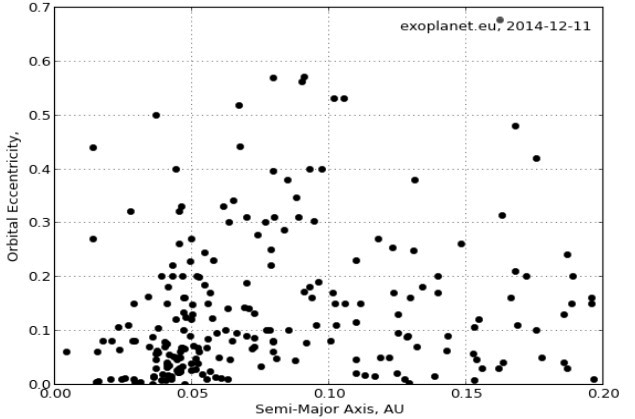
\includegraphics[width=(0.8\textwidth),height=\textheight,keepaspectratio]{e-a}
\caption{Eccentricit\'a vs semiasse.}
\end{figure}

\begin{figure}[!ht]
\centering
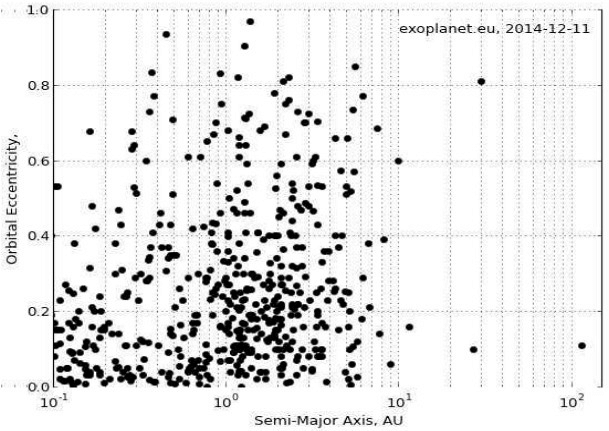
\includegraphics[width=(0.8\textwidth),height=\textheight,keepaspectratio]{e-adistant}
\caption{Eccentricit\'a vs semiasse sistemi distanti.}
\end{figure}

\clearpage

\subsection{Confronto con modelli di formazione sistema solare.}

Modello dominante: aggregazione di pianeti partendo nuclei solidi di polvere o ghiaccio presenti nella nebulosa proto solare.

Pianeti giaganti in posizioni non arbitrarie: oltre l'orbita di Marte.

Processi migrazione planetaria:
\begin{itemize}
    \item Interazione disco proto-planetario/pianeta
    \item Jumping jupiters (:orbite eccentriche??)
    \item A distanza troppo piccola l'interazione mareale stella-pianeta induce forte circolarizzazione delle orbite.
\end{itemize}


\chapter{Galassie. Universo extra-galattico.}
Le galassie; metodi di stima delle distanze; il diagramma di Hubble e considerazioni generali.

L'universo extragalattico: distribuzione della brillanza. Nuclei attivi, quasars. Introduzione alla radioastronomia.
L'universo extragalattico (conclusione). 
\PartialToc

%https://en.wikipedia.org/wiki/Galaxy_morphological_classification

\section{Problematiche: nubi interstellari, galassie.}


Hubble scopri\'e variabili di tipo Cefeidi in Andromeda ed in altre galassie a spirale: parte degli oggetti estesi osservabile erano galassie a grande distanza.

Oggetti estesi osservabili:
\begin{itemize}
\item Nubi interstellari galattiche:
    
hanno estensione di qualche \si{\parsec} e distanza qualche \si{\kilo\parsec}.
\item Galassie:
    
hanno estensione di qualche \si{\kilo\parsec} e distanze maggiori del \si{\mega\parsec} (dimensioni angolari: minuti-gradi).
\end{itemize}

Hubble stima la distanza applicando la relazione $\Pi-L$ delle Cefeidi e altre stelle pulsanti con $\Pi\approx1^d$.

\subsection{Osservabilit\'a di una stella pulsante in una galassia esterna.}

Limiti da Terra:
\begin{itemize}
\item Potere risolutivo ottico del telescopio $\frac{\lambda}{D}$.
\item Seeing atmosferico: risoluzione massima \SI{1}{\arcsec}.
\end{itemize}

Fondo stellare galattico.

Le dimensioni trasversali di un parallelepipedo di base quadrata con dimensioni sulla sfera celeste di $\SI{1}{\arcsec}\times\SI{1}{\arcsec}$ aumentano in maniera proporzionale a $r^2$.

La luminosit\'a assoluta risulta dalla somma su tutte le sorgenti luminose presenti in quel volume e quindi a parit\'a di tipologia di oggetto osservato aumenta come $r^2$: bilancia la diminuzione di luminosit\'a osservata come $\frac{1}{r^2}$.

\begin{definition}{Brillanza di una galassia.}
Magnitudine apparente della minima superficie risolta.
\end{definition}

Fatti:

La brillanza di una galassia \'e indipendente dalla distanza.

\subsubsection{Toy model di galassia.}

Direzione di osservazione parallela all'asse polare della galassia e distanza dalla galassia \SI{1}{\mega\parsec}.

\num{e10} Soli distribuiti su un disco di \SI{10}{\kilo\parsec} di raggio.

In un quadrato $\ang{;;1}\times\ang{;;1}$ osserviamo le stelle nel parallelepipedo di altezza pari allo spessore del disco e come alto di base \mblock{\SI{1}{\mega\parsec}*(\frac{\ang{;;1}}{\SI{1}{\radian}})=\SI{5}{\parsec}} che comprende una frazione \mblock{\frac{25}{\pi\num{e8}}\approx\num{e-7}} delle stelle totali cio\'e circa \num{e3} stelle. A distanza di \SI{1}{\mega\parsec}
\begin{equation*}
    m_{V\odot}=M_{V\odot}+5\log{\frac{\SI{1}{\mega\parsec}}{\SI{10}{\parsec}}}\approx29.7
\end{equation*}

la magnitudine apparente di \num{e3} stelle sarebbe 

\begin{equation*}
m_V=29.7-2.5\log{1000}=22
\end{equation*}

valore realistico per zone non troppo centrali o periferiche.

Una stelle di magnitudine 22 pu\'o corrispondere a una stella di $M_V=-3$ a \SI{1}{\mega\parsec} o $M_V=-8$ a \SI{10}{\mega\parsec}.

Fatti:
\begin{itemize}
    \item L'osservazione di Cefeidi da Terra \'e possibile fino a distanze dell'ordine di \si{\mega\parsec}.
    \item Un fattore 10 in risoluzione fa guadagnare un fattore 100 in luminosit\'a equivalente a 5 magnitudini.
    \item La luce proveniente da una stella simile al Sole a \SI{1}{\mega\parsec} \'e molto minore di un fotone al secondo.
\end{itemize}


\subsection{Misura distanza tramite candela campione.}

\begin{itemize}
    \item Uso di supernovae di tipo I come candela campione. Assunzione: In ogni galassia la stella variabile pi\'u luminosa ha la stessa luminosit\'a assoluta.
    
    Evento raro.
    
    Misura desine di \si{\mega\parsec}.
    \item Le galassie hanno tutte la stessa luminosit\'a.
    \item Le galassie pi\'u luminose di ciascun cluster hanno la stessa luminasit\'a: nelle zone centrali degli ammassi pi\'u grandi fenomeni di merging danno vita ad oggetti massicci e luminosi in maniera anomala.
\end{itemize}

\section{Propriet\'a complessive delle galassie.}
Vedi: The mass distribution in the galactic disc – I. A technique to determine the integral surface mass density of the disc near the Sun.
\subsection{Dispersione della velocit\'a delle stelle.}

La velocit\'a delle stelle \'e legata tramite il viriale al potenziale gravitazionale e quindi alla massa totale

\subsection{Relazioni di Tully-Fisher.}

Relazioni $V/L$.

\subsection{Correzione di Baade per la distanza delle galassie vicine.}

Le dimensioni delle galassie vicine sono paragonabili alla nostra.

Sono presenti tipi diversi di Cefeidi con differenti relazioni $\Pi/L$.

\section{Classificazione delle galassie. Luminosit\'a e spettroscopia.}

\subsection{Diagramma di Hubble.}

\begin{figure}[!ht]
\centering
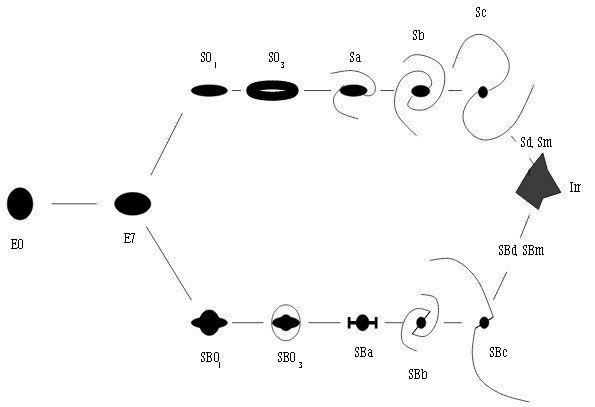
\includegraphics[width=(0.8\textwidth),height=\textheight,keepaspectratio]{galaxiesH}
\caption{Diagramma di Hubble.}
\end{figure}

Fatti:
\begin{itemize}
    \item Ellittiche: E.
    
    Le ellittiche son caratterizzate dal numero \mblock{n=10(1-\frac{b}{c})}, dove b e csono gli assi apparenti dell'ellissi proiezione.
    
    \item Le S0 si distinguono dalle ellittiche per una pi\'u lenta decrescita della luminosit\'a al di fuori della zona centrale: struttura esterna appiattita.
    
    \item Le spirali S sono caratterizzate da una struttura a disco articolata in bracci di maggiore addensamento stellare. Le lettere a,b,c indicano una minor importanza del nucleo centrale e crescente apertura delle braccia (nelle quali si individuano meglio $HII$ regions).
\end{itemize}

\clearpage

\subsection{Classificazione di Yerkers.}

\begin{itemize}
\item B	Barred spirals.
\item D	Galaxies with rotational symmetry but showing neither spiral structure nor ellipticity.
\item cD	Supergiant D galaxies, predominantly found in clusters and embedded in an extensive halo.
\item db	Dumb-bell systems.
\item E	Ellipticals.
\item Ep	Peculiar ellipticals containing conspicuous absorbtion patches.
\item I	Irregulars.
\item L	Low-surface-brightness systems.
\item N	High-luminosity nucleus superimposed on a considerably fainter outer envelope.
\item Q	Quasi-stellar objects.
\item S	Ordinary spirals.
\end{itemize}


\subsection{Spettroscopia delle galassie.}

Il tipo spettrale di una galassia \'e determinato dal tipo spettrale medio delle stelle cha ne fanno parte e dai contributi della materia diffusa e dall'arrossamento interstellare.

Nel diagramma di Hubble abbiamo le ellittiche con stelle di tipo K: $(B-V)\approx1$, spirali con stelle di tipo F e irregolari con stelle di tipo A.

Nelle galassie irregolari sono presenti abbondanti processi di formazione stellare recenti, scarsi nelle ellittiche.

Le righe spettrali sono disperse a causa dell'effetto Doppler: il moto orbitale (solo in parte Kepleriano) \'e caratterizzato da $v\approx\SI{100}{\kilo\meter\per\second}$ (l'effetto pu\'o essere ridotto se l'osservazione \'e localizzatain una regione con velocit\'a relative piccole).

\subsection{Distribuzione spaziale della luminosit\'a.}

Considero la galassia come un gas di stelle.

\begin{definition}{Brillanza superficiale (galassia).}
Luminosit\'a per angolo solido: $\mu=\si{\magnitude\per\squared\arcsec}$.
\end{definition}

La brillanza non dipende dalla distanza.

\begin{itemize}
    \item Galassie giganti: $\mu_B\approx17$.
    \item Galassie medie: $\mu_B\approx22$.
    \item Fondo cielo: $\mu>26$.
\end{itemize}

\begin{definition}{Magnitudine totale (galassia).}
La magnitudine totale della galassia \'e data dall'integrazione del profilo di brillanza fino all'isofota del fondo.
\end{definition}

Magnitudini assolute:
\begin{itemize}
    \item Galassie giganti: $M_V\approx\numrange{-20}{-25}$.
    \item Galassie nane: $M_V\approx\numrange{-15}{-10}$.
\end{itemize}
Si ottengono determinando la distanza tramite candele standard o legge di Hubble (Red Shift).

Determinazione raggio.

Isofota critica definisce il raggio di Holmberg a $\SI{26.5}{\magnitude\per\square\arcsec}$.


\subsection{Profilo di brillanza delle galassie ellittiche.}

\subsubsection{Galassie ellittiche nane.}

Il profilo delle galassie ellittiche nane \'e simile a quello degli ammassi globulari: curve di King.

Le curve di King  sono ottenute mediante modello teorico per il gas di stelle e quindi la distribuzione risultante da una proiezione sulla sfera celeste.

Le curve di King costituiscono una famiglia a 3 parametri:

\begin{align*}
&\Sigma_0,\ r_c&\intertext{ sono la brillanza centrale e il raggio del nucleo definito da $\Sigma(r_c)=\frac{\Sigma_0}{2}$, entrambi osservati e definito il raggio per cui $\Sigma(r_T)=0$}\\
c=\log{\frac{r_T}{r_c}}&\intertext{ricavato tramite best fit.}
\end{align*}

Per c piccolo la distribuzione di massa \'e rapidamente troncata, per c infinitamente grande si ha una distribuzione di massa che va a zero asintoticamente (sfera isoterma).

\subsubsection{Galassie ellittiche giganti.}

La situazione \'e pi\'u complessa. Formula empirica di de Vaucoulurs
\begin{equation*}
\Sigma(r)=\Sigma_e10\expy{-3.33[(\frac{r}{r_e})\expy{\frac{1}{4}}-1]}
\end{equation*}
$r_e$ \'e il raggio efficace determinato attraverso la mediana della distribuzione di brillanza
\begin{equation*}
2\int_0^{r_e}\Sigma(r)2\pi r\,dr=7.22\pi r_e^2\Sigma_e
\end{equation*}
con $\Sigma_e=\Sigma(r_e)$.

Generalizzazione: $\frac{1}{4}\to\frac{1}{n}$ diverso da galassia a galassia.

\subsection{Profilo di brillanza delle galassie a spirale.}

Somma di due componenti:
\begin{itemize}
    \item Bulge (nucleo): andamento alla de Vaucouleurs
    \item Contributo del disco: $\Sigma(r)=\Sigma(r_s)\exp{-\frac{r}{r_s}}$.
\end{itemize}

Il rapporto tra emissione del disco e del bulge \'e $\frac{D}{B}=0.28(\frac{r_s}{r_e})^2\frac{\Sigma(r_s)}{\Sigma_e}$.

\section{Radio-Galassie e quasar.}

\subsection{Galassie di Seyfert.}

Forti righe di emissione.

\subsection{Galssie N.}

Nucelo molto pi\'u brilante del resto.

\subsection{BL Lacertae.}

Visibili solo i nuclei.

\subsection{QSO: quasi-stellar object. Quasar}

Emissione radio \'e legata ad intensi campi EM e a processi tipo radiazione di sincrotrone. Emissione non termica.

La brillanza radio non \'e correlata a quella ottica.

Zone emissione radio: strutture anche estese circostanti il nucleo galattico.

\subsubsection{Quasar}

Le quasar sono oggetti estremamente luminosi e distanti.

Fotometria: eccesso ultravioletto ed infrarosso (non presente in nane bianche o in variabili irregolari).

Spettroscopia: alto red-shift legato all'espansione dell'universo.

\section{Struttura dell'universo su grande scala.}

Cosmolgia: galassie sono le particelle fondamentali, studia la geometria spazio-temporale e la distribuzione di materia nello spazio.

\subsection{Legge di Hubble.}

Chiamo $\vec{r}$ la posizione dell'osservatore, $\vec{v}$ la velocit\'a relativa all'osservatore della sorgente, il vettore $\vec{\phi}$ termine di velocit\'a peculiare della sorgente sofrapposto al flusso di Hubble:
\begin{equation*}
    \vec{v}=H\vec{r}+\vec{\phi}
\end{equation*}
$H$ \'e la costante di Hubble dimensioni di \si{\per\second}: $H\approx\frac{1}{\tau_U}\SI{e-10}{\year}$, usualmente misurata in \si{\kilo\meter\per\second\per\mega\parsec}, $H=\SIrange{60}{70}{\kilo\meter\per\second\per\mega\parsec}$.

Il temine peculiare \'e di entita\'a limitata: per oggetti di stanti pi\'u di \SI{10}{\mega\parsec} il termine di espansione domina sul peculiare $\vec{v}\propto\vec{r}$.

\subsection{Organizzazione gerarchica delle disomogeneit\'a.}

L'universo diventa pi\'u omogeneo all'aumentare della scale: il contrasto di densit\'a tra varie regioni tende a diminuire. Un modello globale ragionevole \'e omogeneo e isotropo.

Organizzazione gerarchica delle disomogeneit\'a:
\begin{enumerate}
\item Galassie.
\item Cluster: ammssi di dimensione intorno al \si{\mega\parsec}.
\item Super-ammassi: scala di \SI{10}{\mega\parsec}.

Filamenti o superfici di densit\'a superiore alla media.
\end{enumerate}

Studio evoluzione sulla base della struttura passata desumibile dalla radiazione di fondo (quando era 1000 volte pi\'u piccolo).

Studio clusterizzazione 3D, esistenza di superfici ad alta densit\'a di galassie e filamenti 1D.

\subsubsection{Termine di correlazione.}

In un volume di universo V ci sono N galassie.

La probabilit\'a di trovare una galassia in $dV$ \'e $P=n\,dV=\frac{N}{V}\,dV$. Per una distribuzione casuale  $P_{12}=n^2\,dV_1\,dV_2$ \'e la probabilit\'a di trovare i volumi $dV_1$ e $dV_2$ popolati.

Per distribuzione non casuale introduco termine di correlazione che per invarianza traslazionale e rotazionale dipende solo dalla distanza tra $dV_1$ e $dV_2$:

\begin{equation*}
    P_{12}=n^2[1+\epsilon(r)]\,dV_1\,dV_2
\end{equation*}

$\epsilon(r)>0$ implica l'esistenza di cluster.

\subsubsection{Toy model: universo quadrato.}

Considero un quadrato di lato L e tutta la materia \'e in quadrato $\frac{L}{4}$:

prendendo un punto a caso $x_1$ la probabilit\'a che sia popolato \'e $\frac{1}{16}$, prendendo un punto $x_2$ a piccola distanza $r\ll l$ \'e probabile che sia nello stesso cluster/regione vuota di $x_1$
\begin{equation*}
    \epsilon(r)=\left\{\begin{array}{cc}
         \frac{1}{16}(256-1)+\frac{15}{16}(-1)=15 & \text{ per } r\ll l \\
         -1 & \text{ per } r\gg l\\
    \end{array}\right.
\end{equation*}

Osservativamente:
\begin{equation*}
    \epsilon_{gal}(r)=(\frac{r}{r_0})\expy{-\gamma}
\end{equation*}
con $r_0\approx\SI{5}{\mega\parsec}$ e $\gamma\approx1.8$. La relazione osservativa conferma struttura clusterizzata con lunghezza di correlazione del'ordine del \si{\mega\parsec}.

Per gli ammassi:
\begin{equation*}
    \epsilon_{cl}(r)=(\frac{r}{r_1})\expy{-\gamma}
\end{equation*}
con $r_1\approx\SI{25}{\mega\parsec}$.

\subsubsection{Test di percolazione.}

Il test di percolazione \'e utile per cercare strutture 1D.

\begin{figure}[!ht]
\centering
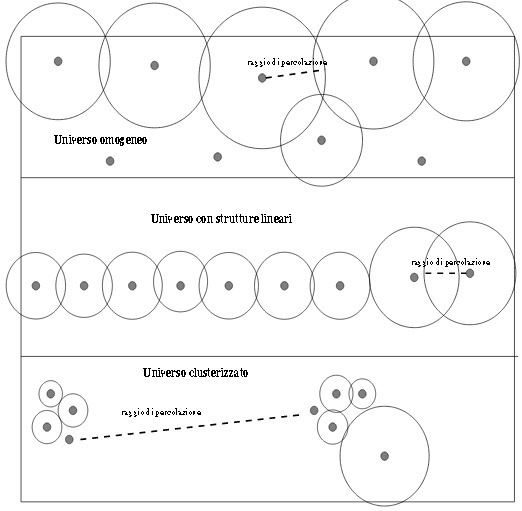
\includegraphics[width=(0.9\textwidth),height=\textheight,keepaspectratio]{percolazione}
\caption{Test di percolazione.}
\end{figure}

Definisco il raggio di percolazione come il raggio per cui preso un insieme di galassie, ognuna circondata da una sfera di tale raggio, ottengo strutture connesse che mi permettono di attraversare il volume dato di universo

\begin{equation*}
    r_{Perc}\left\{\begin{array}{cc}
                =n\expy{-\frac{1}{3}}&\text{distribuzione uniforme}\\
                >n\expy{-\frac{1}{3}}&\text{Cluster}\\
                <n\expy{-\frac{1}{3}}&\text{Struttura 1D o 2D.}\\
    \end{array}\right.
\end{equation*}

\clearpage

\end{document}